\begin{pregunta}
\begin{cuerpo}
 Se desea calcular el m\'inimo de la funci\'on $f(x)=\cos(x^2+1)$ en el intervalo $[0,2]$, cuya gr\'afica, a saber, es:
\medskip

\centerline{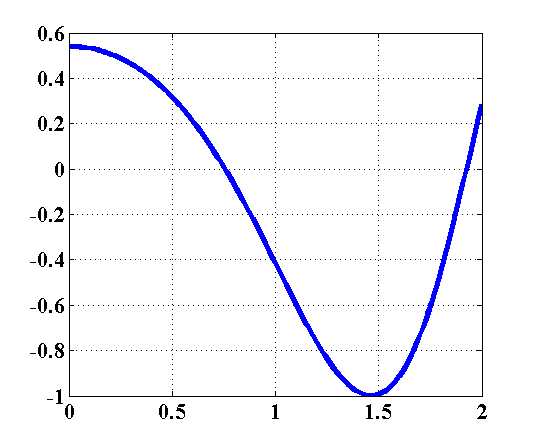
\includegraphics[width=.7\textwidth]{./img/prob01.png}}
\medskip

>Cu\'al de las siguientes instruciones en \textsc{Matlab} calcula una aproximaci\'on del m\'inimo de esta funci\'on?
\end{cuerpo}

\begin{multicols}{2}
\begin{alternativas}
{\begin{tabular}{|p{6cm}|} \hline \verb"f=inline('-2*x.*sin(x.\^{}2+1)');"\\ \verb"fmin=fzero(f,1.5)"\\ \hline \end{tabular}}
{\begin{tabular}{|p{6cm}|} \hline \verb"f=inline('-2*x.*sin(x.\^{}2+1)');"\\ \verb"fmin=quad(f,1.5)"\\ \hline \end{tabular}}
{\begin{tabular}{|p{6cm}|} \hline \verb"f=inline('cos(x.\^{}2+1)');"\\ \verb"fmin=min(f)"\\ \hline \end{tabular}}
{\begin{tabular}{|p{6cm}|} \hline \verb"f=inline('cos(x.\^{}2+1)');"\\ \verb"fmin=fzero(f,1.5)"\\ \hline \end{tabular}}
\end{alternativas}
\end{multicols}
\justificacion{0cm}
\end{pregunta}